\section{Continuous Symmetries}
\label{s:symm}

\subsection{Definitions}

A dynamical system, $\dot{\ssp}=\vel(\ssp)$, is \emph{equivariant} under a continuous
symmetry transformation
\beq
	\ssp'= \LieEl (\theta) \ssp = \exp\left( \theta \Lg\right)\ssp,
\ee{contSymTrans}
if the condition
$\vel(\LieEl (\theta) \ssp ) = \LieEl (\theta) \vel( \ssp ) $
or equivalently \rf{DasBuch}
\beq
  \groupTan(\vel)  - \Mvar(\ssp) \, \groupTan(\ssp) =0
  \,,
\ee{inftmInv}
is satisfied for every point of its \statesp . In equations \refeq{contSymTrans}
and \refeq{inftmInv}, $\LieEl (\theta)$ is the Lie group element, $\Lg$
is the Lie algebra generator, $\Mvar(\ssp)_{ij} = {\pde \vel_i}/{\pde\ssp_j} |_x$
is the \stabmat , $ \groupTan(\ssp) = \Lg \ssp $ is the group tangent evaluated
at the point $\ssp$ , and $ \groupTan(\vel) = \Lg \vel(\ssp) $ is the group
tangent for the velocity vector evaluated at \ssp. 
\DB{}{The notation $\groupTan(\vel) = \Lg \vel(\ssp)$ and $\groupTan(\ssp) = \Lg \ssp$ is really cofusing. Is there a particular reason we are using it here?}
\ES{}{There is also a notational conflict between time $t$ and $\groupTan$, so that we have expressions like $\groupTan(\ssp)$ and $\ssp(t)$.
Burak, please fix this by making a consistent choice.}
\BB{}{I'm working on producing results, please have a look at \refref{BudCvi14} 
fix these following the conventions we used there.}

\label{s:relatives}

If the dynamical orbit of a point $\ssp_\stagn$ coincides with its group
orbit, namely if one can find a group parameter $\theta (t)$, for every point $\ssp (t)$
on the orbit of $\ssp_\stagn$ such that
\beq
  \ssp (t) = \ssp_\stagn + \int_0^t d\tau \vel(\ssp (\tau)) = \LieEl (\theta (t)) \ssp_\stagn
  \, ,
\ee{releq}
 $\ssp_\stagn$ is called a \emph{ \reqv }. By expanding both sides of \refeq{releq}
for infinitesimal time, we can get the relation
$\vel(\ssp_\stagn) = \dot{\theta}(\ssp_\stagn) \Lg \ssp_\stagn$,
and since this has to hold for every point on the group orbit of $\ssp_\stagn$
we deduce that $\dot{\theta} = c$ is a constant. We now can multiply the equivariance
condition \refeq{inftmInv} evaluated at the \reqv\ by $c$ and write the
\reqv\ condition compactly as
\beq
(\velRel \Lg - \Mvar ) \vel (\ssp_\stagn) =0
\,.
\ee{ReqvMargEig}
The constant group parameter velocity $c$  is called the \phaseVel .

We define the  \emph{ \rpo} as a \statesp\ point $\ssp_\rpprime$ which satisfies
\beq
  \ssp (T) = \ssp_\rpprime  + \int_0^T d\tau \vel(\ssp (\tau)) = \LieEl (\theta_\rpprime ) \ssp_\rpprime
  \,,
\ee{relpo}
meaning that the trajectory of $\ssp_\rpprime$ intersects its group orbit at
time $T$. While the trajectory of a \rpo\ traces out the same path shifted
by the group action over and over again, as we shall see in the examples of
\ref{s:twoModeSymRed}, such a trajectory can be very complicated if the
continuous symmetry of the system is not reduced.

\subsection{\Mslices}
\label{s-slice}

A \emph{\slice} \pSRed\ is a codimension $N$ submanifold that is cut
by every group orbit once and only once, where $N$ is the number of continuous
symmetries in presence. In \emph{\mslices}, one represents the solution
of a $d$-\dmn\ dynamical system as a solution $\sspRed (t)$ within the
$(d-N)$-\dmn\ \slice\  and $N$ time dependent group parameters $\theta(t)$
that maps $\sspRed (t)$ to the full \statesp\ by the group action $\LieEl(\theta(t))$.
While this definition does not make any restriction on the shape of the
\slice, in practice, a linear condition is constructed by picking a
particular
\template\ ($\slicep$) and defining the \slicePlane\ as the hyperplane
that involves the \template\ $\slicep$ and is perpendicular to the group
tangent evaluated at this template $\sliceTan{} = \groupTan(\slicep) = \Lg \slicep$.
\SlicePlane\ and reduced trajectories are illustrated in \reffig{f-ReducTraj1}.

%% ReducTraj*.* - read dasbuch/book/FigSrc/inkscape/00ReadMe.txt
\begin{figure}
\begin{center}
 \setlength{\unitlength}{0.40\textwidth}
 %% \unitlength = units used in the Picture Environment
 \begin{picture}(1,0.8361641)%
   \put(0,0){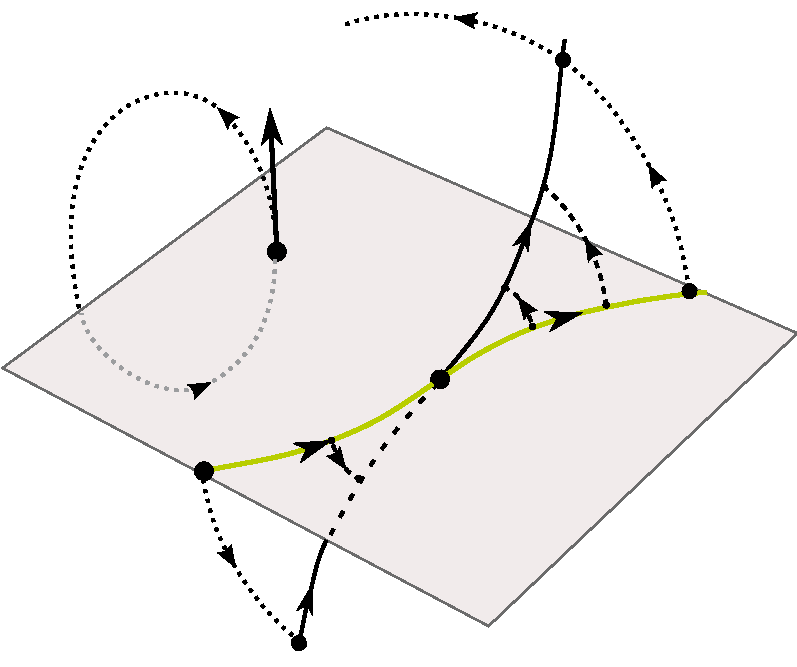
\includegraphics[width=\unitlength]{ReducTraj5.pdf}}%
   \put(0.09054399,0.38282057){\color[rgb]{0,0,0}\rotatebox{-30.34758661}{\makebox(0,0)[lb]{\smash{$\pSRed$}}}}%
   \put(0.57768586,0.29773425){\color[rgb]{0,0,0}\rotatebox{0.0313674}{\makebox(0,0)[lb]{\smash{$\sspRed(0)$}}}}%
   \put(0.59310014,0.69932675){\color[rgb]{0,0,0}\rotatebox{0.03136739}{\makebox(0,0)[lb]{\smash{$\ssp(\tau)$}}}}%
   \put(0.8268425,0.39772328){\color[rgb]{0,0,0}\rotatebox{0.03136739}{\makebox(0,0)[lb]{\smash{$\sspRed(\tau)$}}}}%
   \put(0.81220962,0.66529577){\color[rgb]{0,0,0}\rotatebox{0.03136739}{\makebox(0,0)[lb]{\smash{$\LieEl(\tau)$}}}}%
   \put(0.23150193,0.63610779){\color[rgb]{0,0,0}\rotatebox{0.0313674}{\makebox(0,0)[lb]{\smash{$\LieEl\,\slicep$}}}}%
   \put(0.37740434,0.49597258){\color[rgb]{0,0,0}\rotatebox{0.0313674}{\makebox(0,0)[lb]{\smash{$\slicep$}}}}%
   \put(0.3627714,0.69665188){\color[rgb]{0,0,0}\rotatebox{0.0313674}{\makebox(0,0)[lb]{\smash{$\sliceTan{}$}}}}%
 \end{picture}%
\end{center}
\caption{\label{f-ReducTraj1}
% (b)
\SlicePlane\ \pSRed\ is a hyperplane % \refeq{PCsect0}
passing through the {\template} point $\slicep$,
and normal to the group tangent $\sliceTan{}$ at $\slicep$.
It intersects all
group orbits (indicated by dotted lines here) in an open
neighborhood of $\slicep$.  The full
\statesp\ trajectory $\ssp(\tau)$ and the \reducedsp\
trajectory $\sspRed(\tau)$ belong to the same group orbit
$\pS_{\ssp(\tau)}$ and are equivalent up to a group rotation
$\LieEl(\gSpace)$ %, defined in   refeq{sspOrbit}
(from \wwwcb{}).
}%
\end{figure}

Reduced trajectories $\sspRed (t)$, can be obtained in two ways: post-processing
or integration within the \slice. In the former, one takes the symmetry
equivariant data and looks for the time dependent group parameter  ($\theta (t)$)
for which the group operation transforms the $\ssp (t)$ to
$\sspRed (t) = \LieEl(- \theta (t)) \ssp (t)$ that satisfies
the \slice\ condition:
\beq
(\sspRed(t) - \slicep)\cdot \sliceTan{} = 0
\,.
\ee{SliceCond}
This method and is applicable to both computer and laboratory experiments.
In the second method, one computes the reduced trajectory $\sspRed (t)$ and
the time dependent group parameter $\theta (t)$ directly by integrating
\bea
\velRed(\sspRed) &=& \vel(\sspRed)
   -\dot{\theta}(\sspRed) \, \groupTan(\sspRed)
\continue
\dot{\theta}(\sspRed) &=& {\braket{\vel(\sspRed)}{\sliceTan{}}}/
               {\braket{\groupTan(\sspRed)}{\sliceTan{}}}
\, ,
\label{eq:so2reduced}
\eea
for Abelian groups. In \refeq{eq:so2reduced}, $\velRed$ is the projection
of the velocity function onto the \slicePlane . For a detailed derivation
of \refeq{eq:so2reduced}, see \refref{DasBuch}. Note that the time derivative
of the group parameter, which appears also in the reduced velocity function,
becomes singular if the dot product $\braket{\groupTan(\sspRed)}{\sliceTan{}}$
vanishes. We will refer the set of points within a \slicePlane\ which satisfies
\beq
\braket{\groupTan(\sspRed^*)}{\sliceTan{}} = 0
\,
\ee{ChartBordCond}
as the \emph{\sliceBord } .

%In general, \chartBord\ can be avoided by use of
%multiple \template s and arranging them in a way that the trajectories do not
%intersect the \chartBord , as done in \refref{atlas12}. In the particular
%case of the \twoMode\ system that we study in this paper, we can describe
%the reduced dynamics using a single \slice\ by picking a \template\ for which
%the \chartBord\ is a flow invariant subspace, hence never visited.

%If a $d$\dmn\ dynamical flow is $\Group$-equivariant under actions of
%an $N$ continuous parameters symmetry group $\Group$, its $d$\dmn\ \statesp\ is foliated
%by $N$\dmn\ group orbits, and the symmetry-\reducedsp\
%$\pS/\Group$ is $(d\!-\!N)$\dmn.
%The simplest continuous symmetry groups are the 1-parameter compact rotation
%group $\SOn{2}$ and the 1-parameter noncompact translation group
%$T(1)$; here we shall focus on the $\SOn{2}$ case.

So far, we have not made any specification on the symmetry group that we
are reducing, other than the Abelian requirement for \refeq{eq:so2reduced}.
From here on, we restrict our discussion to 1-parameter compact $\SOn{2}$
rotations which arise in spatially extended systems. In order to construct
a representation for $\SOn{2}$ let us take a Fourier series expansion of
a real valued smooth periodic function:
\beq
	u(\phi) = a_0 + \sum\limits_{k=- \infty}^\infty a_k e^{i k \phi} .
\ee{FourierSeries}
Truncating the expansion to $m$ modes we
write the real and imaginary parts of the Fourier coefficients with
$k \geq 1$ in a state vector $(x_1, y_1, x_2, y_2,..., x_m, y_m)$, where
$a_i = x_i + i y_i$, and represent the $\SOn{2}$ group action on this vector
as a block diagonal matrix:
%More explicit form, does not fit in a column:
%\beq
	 %\LieEl (\theta)= \\
					  %\begin{pmatrix}
					  %\cos \theta & \sin \theta & 0               & 0              & \cdots & 0              & 0               \\
					 %-\sin \theta & \cos \theta & 0               & 0              & \cdots & 0              & 0               \\
					  %0             & 0 		   & \cos 2 \theta & \sin 2 \theta & \cdots & 0              & 0               \\
					  %0             & 0            &-\sin 2 \theta & \cos 2 \theta & \cdots & 0              & 0               \\
					  %\vdots       & \vdots      & \vdots         & \vdots        & \ddots & \vdots         & \vdots         \\
					  %0             & 0 		   & 0               & 0              & \cdots & \cos m \theta & \sin m \theta  \\
					  %0             & 0            & 0	             & 0              & \cdots &-\sin m \theta & \cos m \theta
					  %\end{pmatrix}
%\eeq
\beq
	\LieEl(\theta) = \begin{pmatrix}
						R(\theta) & 0 			  & \cdots & 0 \\
						0		   & R(2 \theta) & \cdots & 0 \\
						\vdots	   & \vdots 	  & \ddots & \vdots \\
						0		   & 0	          & \cdots & R (m \theta)
					   \end{pmatrix} ,
\ee{mmodeLieEl}
and
\beq
	R(n \theta) =	\begin{pmatrix}
					\cos n \theta & - \sin n \theta \\
					\sin n \theta & \cos n \theta
					\end{pmatrix}
\ee{rotationmatrix}
is the rotation matrix for $n$th Fourier mode.
The Lie algebra generator is
\beq
	 \Lg =  \begin{pmatrix}
			 0 & -1 & 0 & 0 & \cdots & 0 & 0 \\
			 1 & 0 & 0 & 0 & \cdots & 0 & 0 \\
			 0 & 0 & 0 & -2 & \cdots & 0 & 0 \\
			 0 & 0 & 2 & 0 & \cdots & 0 & 0 \\
			 \vdots & \vdots & \vdots & \vdots & \ddots & \vdots & \vdots \\
			 0 & 0 & 0 & 0 & \cdots & 0 & -m \\
			 0 & 0 & 0 & 0 & \cdots & m & 0
			 \end{pmatrix} .
\ee{mmodeLg}
Now let us consider the following specific choice of a \slice\ \template\:
\beq
	\slicep = (1, 0, ..., 0) .
\ee{firstmodetemp}
Eq.~\refeq{SliceCond} restricts the points on the hyperplane defined
by the template point \refeq{slicetemp} to the following form:
\beq
	\sspRed = (\hat{x}_1, 0, \hat{x}_2, \hat{y}_2, ..., \hat{x}_m, \hat{y}_m) .
\ee{slicetemp}
These points satisfy the \sliceBord\ condition \refeq{ChartBordCond} only
if $\hat{x}_1 = 0$, in other words, as long as the first mode magnitude is
non zero, there is a corresponding unique point to every group orbit on the
\slicePlane\ defined by \refeq{firstmodetemp}. We pick the \slice\ \template\
\refeq{firstmodetemp} for computational convenience, in general, any first
mode template $\slicep = (x_1, y_1, 0,...,0)$ would do as good since the
first mode has the symmetry of a circle. We also restrict the \slicePlane\
to the half-space where $x_1 > 0$ to have a unique representative point for
each group orbit since otherwise each group orbit pierces the \slicePlane\
twice.

The \template\ \refeq{firstmodetemp} for $\SOn{2}$ was introduced in \refref{BudCvi14}
and is different than the ones that were used in the previous implementations
\rf{rowley_reconstruction_2000,BeTh04,SiCvi10,FrCv11,atlas12,ACHKW11}
of the \mslices, in the sense that it is solely geometrical and it does
not necessarily carry any information about the dynamics. More insight is
gained by writing the reduced evolution equations \refeq{eq:so2reduced}
explicitly for the template \refeq{firstmodetemp}:
\bea
\velRed ( \sspRed )          &=& \vel(\sspRed)
   - \frac{\vel(\sspRed)_2}{\sspRed_1} \, \groupTan(\sspRed)
\label{e-so2red1stmode}
\,.
\eea
\ES{}{$\vel(\sspRed)_2$ has not been introduced and is very confusing. I would suggest
using the notation of BudCvi14.tex: state space point is $a$, real variables are
$x_i$ and $y_i$ and right velocity components explicitly.
}
In order to regulate the near-divergent behavior of the velocity function
in \refeq{e-so2red1stmode} close to $\sspRed_1 = \sspRed_2 = 0$, rescaled time variable
$d \tau = dt / \sspRed_1$ was defined in \refref{BudCvi14}. While rescaling
time is essential for resolving the orbits during close passages to
$\sspRed_1 = 0$, in the study of the \twoMode\ system, we will omit this
step since the vanishing 1st mode corresponds to the invariant subspace of
the flow and hence is never visited by the dynamics.

\subsection{Postproccessing approach}
\label{s-slice2modes}
\ES{}{This section is a regression to the ``method of moving frames'' (postprocessing approach)
and as such belongs here. It has to be generalized a bit (I will do it if you agree with the change}. 
Second mode slice can be used also for integration on the slice and can be introduced earlier.
}

\begin{figure}%[H]
\centering
 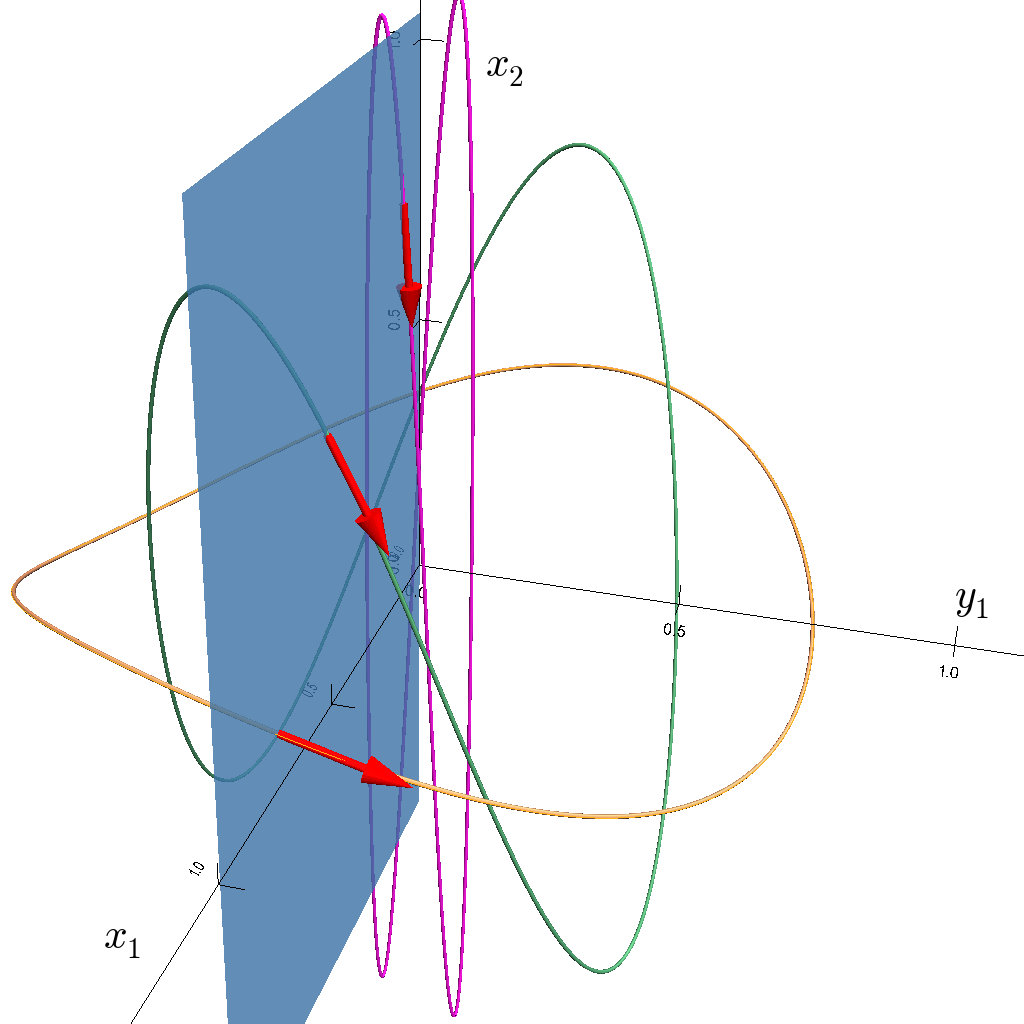
\includegraphics[width=0.45\textwidth]{BBgorbitsandslice}
\caption{$\SOn{2}$ Group orbits of $(0.75, 0, 0.1, 0.1)$ (orange), $(0.5, 0, 0.5, 0.5)$ (green)
$(0.1, 0, 0.75, 0.75)$ (pink) of two Fourier modes and the first mode \slicePlane\
projected on three dimensions. 3D projections of the group tangents at the
intersections with the \slicePlane\ are shown as red arrows.}
\label{fig:BBgorbitsandslice}
\end{figure}

In \refsect{s-slice}, we explained the general procedure for reducing
the \SOn{2} symmetry by \mslices, here, we are going to focus on its
geometrical interpretation by narrowing the consideration down to the \twoMode\
system. The \slice\ defined by \refeq{firstmodetemp} and the direction
constraint $x_1 > 0$ fixes the phase of the first complex Fourier mode to $0$;
and the \statesp\ points are related to their \slice\ ``representatives''
by the following $\Un{1}$ action:
\beq
	\sspRedC_n = e^{-\ii n \phi_1} \sspC_n \, .
\ee{e-1stmodeTransform}
We immediately see that the reconstruction phase in \refeq{eq:so2reduced}
is, for this particular \slice, the phase of the first mode without the
symmetry reduction. The relation \refeq{e-1stmodeTransform} provides us
another interpretation for the \sliceBord :  For the template \refeq{firstmodetemp},
\sliceBord\ condition \refeq{ChartBordCond} yields,
$|\sspRedC_1| = |\sspC_1| = 0$, this means that the phase of the first Fourier
mode is not defined, hence the transformation \refeq{e-1stmodeTransform}
has no meaning. We illustrated this by drawing the $3D$ projections of the
group orbits, and group tangents of three reduced \statesp\ points in
\reffig{fig:BBgorbitsandslice}. Note, in \reffig{fig:BBgorbitsandslice}
that as the magnitude of the first mode, $\sqrt{x_1^2 + y_1^2}$, relative
to that of the second mode becomes smaller, its respective group tangent
has a larger component that lies within the \slice; \sliceBord\ condition
\refeq{ChartBordCond} is satisfies when the group tangent is entirely in the \slice.

An immediate generalization of the transformation \refeq{e-1stmodeTransform},
can be fixing the phase of the higher Fourier modes; this, however, requires
some extra care as we shall explain for the second Fourier mode next.
Consider the phase-fixing transformation,
\beq
	\sspRedC_n = e^{-\ii n \phi_2/2} \sspC_n \, ,
	\label{e-2ndmodeTransform}
\eeq
which would fix the phase of $\sspRedC_2$ to $0$. Note, however, that
$\phi_2 \in (0, 2 \pi]$ in can have discontinuities of $2 \pi$, and this
would translate to the transformation of the first Fourier mode by \refeq{e-2ndmodeTransform}
as a phase discontinuity of $\pi$. This discontinuity can be fixed by another
transformation:
\bea
	\tilde{\sspC}_1 &=& e^{-\ii 2 \hat{\phi}_1} |\sspRedC_1 | \, , \continue
	\tilde{\sspC}_{n \neq 1} &=& \sspRedC_n \, ,
	\label{e-PhaseDoubling}
\eea
where we simply doubled the phase $\hat{\phi}_1$ of the symmetry-reduced
first mode $\sspRedC_1$, obtained by \refeq{e-2ndmodeTransform} and left
the rest of the modes unchanged. Combination of \refeq{e-2ndmodeTransform}
and \refeq{e-PhaseDoubling} is a valid symmetry reduction scheme since every
group orbit is represented by a single point, furthermore, it is also continuous
and revertible hence one can make further computations, such as constructing
Poincar\'{e} sections, using this form. For the 2-mode case at hand, representation
\refeq{e-PhaseDoubling} does not have any particular advantage against
\refeq{e-1stmodeTransform}, however, for higher dimensional flows, second
(or higher) Fourier mode subspaces can have dynamical importance as shown in
\refref{SCD07}. In order to capture those regions of the \statesp\ this
representation would be a useful alternative.

\subsection{Polar coordinates}
\label{s-polar}

In \refref{PoKno05}, a polar coordinate representation of \refeq{eq:DangSO2}
is obtained by defining the $\LieEl$-invariant phase: $\Phi = \phi_2 - 2 \phi_1$
and three symmetry invariant coordinates $(r_1, r_2 \cos \Phi, r_2 \sin \Phi)$.
One can see by direct comparison with \refeq{e-1stmodeTransform}, which
yields $\sspRedC_1 = r_1$ and $\sspRedC_2 = r_2 e^{\ii \Phi}$, that this
representation is a special case $(m=2)$, of the \slice\ defined by
\refeq{firstmodetemp}. Corresponding ODEs for the polar representation
were obtained in \refref{PoKno05} by  chain rule and substitution. Note
that \mslices\ provides a general form \refeq{e-so2red1stmode} for symmetry
reduced time evolution.

